\documentclass{article}
\usepackage{graphicx}
\usepackage[style=ieee]{biblatex} % Establecer el estilo de las referencias como IEEE
\usepackage{xcolor}
\usepackage{hyperref}
\usepackage{titletoc}
\usepackage{adjustbox}
\usepackage[spanish]{babel}

\hypersetup{
    colorlinks=true,
    linkcolor=blue, % Color del texto del enlace
    urlcolor=blue % Color del enlace
}

\usepackage{longtable} % Agrega el paquete longtable

\definecolor{mygreen}{RGB}{0,128,0}

\usepackage{array} % Para personalizar la tabla
\usepackage{booktabs} % Para líneas horizontales de mejor calidad
\usepackage{graphicx} % Paquete para incluir imágenes
\usepackage{float}
\usepackage[section]{placeins}

% Definir márgenes
\usepackage[margin=1in]{geometry}

\renewcommand{\contentsname}{\textcolor{mygreen}{Tabla de Contenidos}}

\begin{document}

\begin{titlepage}
    \centering
    % Logo de la Universidad
    
\includegraphics[width=0.48\textwidth]{logo_universidad.png}
    \par\vspace{2cm}

    % Nombre de la Universidad y detalles del curso
    {\Large \textbf{Universidad Nacional de Colombia} \par}
    \vspace{0.5cm}
    {\large Ingeniería de Sistemas y Computación \par}
    {\large 2025966 Lenguajes de Programación (02)\par}
    \vspace{3cm}

    % Detalles del laboratorio y actividad
    {\large \textbf{Tarea 24} \par}
    {\large Completar, compilar y ejecutar el analizador para la estructura de selección.\par}
    \vspace{3cm}

    % Lista de integrantes
    {\large \textbf{Integrantes:} \par}
    \vspace{0.5cm}
    \begin{tabular}{ll}
    Javier Andrés Tarazona Jiménez & jtarazonaj@unal.edu.co \\
    Eder  José Hernández Buelvas   & ehernandezbu@unal.edu.co \\
    Juan Sebastián Muñoz Lemus     & jumunozle@unal.edu.co   \\
    David Felipe Marin Rosas       & dmarinro@unal.edu.co   \\
    \end{tabular}
    \par\vspace{3cm}

    % Fecha
    {\large Mayo 7 de 2025 \par}
\end{titlepage}

\tableofcontents % Inserta la tabla de contenidos

\newpage % Salto de página para separar la tabla de contenidos del contenido del documento

% Contenido del artículo----------------------------------------------------------

%---------------------------------------------------------------------------------
% Intro --------------------------------------------------------------------------
%---------------------------------------------------------------------------------

\section{Introducción}\label{sec:intr}

Este documento aborda el desarrollo y comprobación de un analizador léxico implementado con FLEX, una herramienta reconocida por su eficiencia en la construcción de analizadores de lenguaje. El objetivo principal es procesar correctamente la estructura de control condicional \texttt{if}, tomando como referencia la explicación presentada en la sección 3.23 del libro \textit{Compilers: Principles, Techniques, and Tools} (segunda edición) de Alfred Aho, Monica Lam, Ravi Sethi y Jeffrey Ullman. Para lograrlo, se parte de un ejemplo extraído del texto, el cual se adapta y completa para garantizar una adecuada identificación de palabras reservadas y su correcto tratamiento durante el análisis.
%---------------------------------------------------------------------------------
% Marco Teórico ------------------------------------------------------------------
%---------------------------------------------------------------------------------

\section{Marco Teórico}\label{sec:marc}

\subsection*{Procesadores de Lenguaje}

Los procesadores de lenguaje son programas diseñados para interpretar, transformar o ejecutar instrucciones escritas en un lenguaje de programación. Entre ellos destacan los compiladores, los intérpretes y los sistemas híbridos, cada uno con métodos y propósitos específicos.

\subsection*{Compiladores}

Un compilador traduce un programa fuente a un programa equivalente en otro lenguaje, generalmente de bajo nivel o código máquina. Durante la compilación, se realiza la detección de errores y la optimización del código para su posterior ejecución. Entre las fases involucradas destacan el preprocesamiento, ensamblaje, vinculación y carga, que aseguran que el resultado final sea ejecutable en la plataforma destino.

\subsection*{Intérpretes}

A diferencia del compilador, un intérprete ejecuta directamente las instrucciones del código fuente en tiempo de ejecución. Esta característica permite diagnósticos de errores más detallados, aunque con una menor velocidad de ejecución comparada con programas compilados.

\subsection*{Procesadores Híbridos}

Algunos lenguajes adoptan un enfoque intermedio, generando primero un código intermedio —como el bytecode en Java— que luego es interpretado o compilado dinámicamente mediante técnicas como la compilación JIT (Just-In-Time), mejorando el rendimiento en tiempo de ejecución.

\subsection*{Estructura de un Compilador}

Un compilador se divide conceptualmente en dos etapas: análisis y síntesis.  
\textbf{El análisis} descompone el código fuente en componentes básicos, detecta errores y construye una representación intermedia. Dentro de esta fase, destacan:
\begin{itemize}
    \item \textbf{Análisis léxico:} Identifica lexemas y los convierte en tokens.
    \item \textbf{Análisis sintáctico:} Organiza los tokens en estructuras gramaticales.
    \item \textbf{Análisis semántico:} Verifica la coherencia de las operaciones.
\end{itemize}

\textbf{La síntesis} genera el código objetivo a partir de la representación intermedia, realizando optimizaciones y adaptando la salida al sistema donde se ejecutará.

\subsection*{Análisis Léxico}

El análisis léxico es la fase inicial de un compilador. Su función es leer el flujo de caracteres del programa y agruparlos en unidades significativas llamadas tokens, eliminando elementos irrelevantes como espacios o comentarios. Cada token encapsula información necesaria para las etapas de análisis sintáctico y semántico.

\subsection*{FLEX}

FLEX es una herramienta que automatiza la creación de analizadores léxicos. A partir de una descripción de patrones, genera código capaz de reconocer tokens, facilitando el desarrollo de compiladores y otros sistemas de procesamiento de texto.

\subsection*{Expresiones y Definiciones Regulares}

Para reconocer patrones léxicos, se emplean expresiones regulares, que describen conjuntos de cadenas válidas. Operaciones como la concatenación, alternación o repetición permiten definir patrones complejos. Las definiciones regulares permiten simplificar y reutilizar estos patrones, evitando redundancia y facilitando la lectura y mantenimiento del analizador.

\subsection{Contextualización del problema}

En el contexto del diseño de compiladores, la correcta segmentación y categorización de los componentes léxicos es la base para una traducción precisa de los programas. Una estructura tan elemental como la instrucción condicional \texttt{if} requiere ser identificada de forma inequívoca, ya que determina el flujo de control de la ejecución. Para ello, se hace necesario implementar un analizador léxico que detecte y clasifique correctamente cada palabra clave, operador y símbolo. Adaptar ejemplos de libros de referencia a entornos de desarrollo actuales permite a los estudiantes enfrentar situaciones reales, resolver incompatibilidades y afianzar habilidades en el manejo de herramientas como FLEX. De esta forma, se garantiza que los programas fuente se traduzcan de forma eficiente y sin ambigüedades, manteniendo la integridad semántica del código.

%---------------------------------------------------------------------------------
% Descripción y Justificación del Problema a Resolver ----------------------------
%---------------------------------------------------------------------------------

\section{Descripción y Justificación del Problema a Resolver}\label{sec:descr}

El trabajo consiste en comprender y adaptar un caso práctico del mencionado libro, utilizando FLEX como generador de analizadores léxicos. Se modificará el código base para asegurar que reconozca de forma efectiva la estructura condicional y clasifique apropiadamente las palabras clave. Una vez finalizadas las modificaciones, el programa se compilará empleando utilidades como \texttt{flex} y \texttt{gcc}, para finalmente someterlo a una serie de pruebas que permitan verificar su desempeño y exactitud.

\subsection{Justificación}

El uso de FLEX resulta fundamental para estudiantes y profesionales de áreas como Ingeniería de Sistemas y Ciencias de la Computación, especialmente aquellos enfocados en la creación de compiladores y herramientas de análisis de lenguajes. Automatizar la generación de analizadores léxicos simplifica una de las etapas más críticas en el diseño de compiladores: la segmentación y clasificación de componentes léxicos. Mediante esta práctica se consolida la teoría aprendida, se adquiere destreza en la solución de problemas de compatibilidad y se fortalece la capacidad de adaptar ejemplos académicos a entornos de desarrollo actuales.


\subsection{Objetivo Principal}

El objetivo principal de este trabajo es diseñar, modificar y validar un analizador léxico capaz de reconocer correctamente la estructura de selección condicional \texttt{if}, utilizando la herramienta FLEX como generador de código. Para ello, se tomará como punto de partida un ejemplo de la sección 3.23 del libro \textit{Compilers: Principles, Techniques, and Tools} (segunda edición) y se adaptará para garantizar una correcta clasificación de palabras reservadas y su procesamiento adecuado dentro del flujo de análisis léxico.
%---------------------------------------------------------------------------------
% Diseño de la solución ---------------------------------------------------------
%---------------------------------------------------------------------------------

\section{Diseño de la solución}\label{sec:dis}

La aplicación desarrollada está orientada a servir como entorno de apoyo para la creación, ajuste y verificación de analizadores léxicos enfocados en estructuras condicionales, en particular la instrucción \texttt{if}. Su diseño responde a objetivos didácticos y de experimentación, brindando a los usuarios una plataforma sencilla para trabajar con FLEX, personalizar patrones léxicos y observar su funcionamiento en diferentes situaciones.

El sistema se estructura de forma modular, dividiendo sus funcionalidades en componentes especializados que facilitan la gestión y mantenimiento del proyecto. Los módulos principales son:

\begin{itemize}
    \item \textbf{Editor de Código:} Proporciona un espacio donde el usuario puede escribir o modificar el archivo fuente en FLEX, validando la correcta definición de patrones y símbolos.
    \item \textbf{Gestor de Compilación:} Automatiza la conversión del archivo FLEX a código C y su posterior compilación mediante herramientas como \texttt{gcc}, generando el ejecutable necesario.
    \item \textbf{Motor de Pruebas:} Permite definir casos de prueba variados para alimentar al analizador léxico, evaluando su respuesta ante diferentes entradas.
    \item \textbf{Visualizador de Resultados:} Organiza y presenta los resultados obtenidos de forma clara, facilitando la comparación entre escenarios de prueba.
\end{itemize}

Cada módulo trabaja de manera coordinada para ofrecer una experiencia interactiva y didáctica, permitiendo iterar rápidamente entre la edición del código, su compilación y la ejecución de pruebas.

\subsection{Metodología}

Para garantizar el funcionamiento correcto de la aplicación, se adoptó una metodología basada en fases bien definidas:

\begin{enumerate}
    \item \textbf{Definición de Constantes y Patrones:} Se organizan las palabras clave y símbolos léxicos en secciones bien delimitadas dentro del archivo FLEX, asegurando su correcta categorización.
    \item \textbf{Edición y Configuración del Código:} Se desarrolla o ajusta el archivo fuente con las expresiones regulares necesarias para reconocer cada token relevante.
    \item \textbf{Generación y Compilación del Analizador:} Se ejecuta el proceso de traducción con \texttt{flex}, obteniendo el código en C, que luego se compila con \texttt{gcc} para producir el ejecutable.
    \item \textbf{Pruebas y Validación:} Se diseñan entradas de prueba representativas que se procesan con el analizador, verificando la correcta identificación de tokens y palabras reservadas.
    \item \textbf{Análisis de Resultados:} Se revisan las salidas generadas para confirmar el funcionamiento del analizador y se realizan ajustes si es necesario, optimizando patrones y definiciones.
\end{enumerate}


%---------------------------------------------------------------------------------
% Código Fuente ---------------------------------------------------------
%---------------------------------------------------------------------------------

\section{Código Fuente}\label{sec:cod}

El código fuente de esta tarea se encuentra adjunto en el buzón 
24 Muñoz Lemus Juan Sebastian 02.zip
y disponible en el repositorio GitHub del proyecto:
\begin{center}
\url{https://github.com/JavierTarazona06/LP02_Tareas/tree/main/Tarea24}
\end{center}
%---------------------------------------------------------------------------------
% Manual Usuario ---------------------------------------------------------
%---------------------------------------------------------------------------------

\section{Manual Usuario}\label{sec:man_u}

Este apartado ofrece una guía básica para la instalación de herramientas, descarga del código fuente y ejecución del analizador léxico desarrollado para esta práctica.

\subsection{Instalación de Herramientas}

Para poder compilar y ejecutar el analizador léxico es indispensable contar con Flex, Bison y un compilador C como MinGW. Para instrucciones detalladas sobre cómo instalar estos componentes, se recomienda consultar el documento de referencia correspondiente a la práctica anterior.

\subsection{Descarga y Preparación del Proyecto}

\begin{enumerate}
    \item Acceda a este enlace \href{https://github.com/JavierTarazona06/LP02_Tareas/tree/main/Tarea24/Code}{Tarea 24}
    \item Descargue los archivos Tarea24.l y Funciones.c
    \item Guarde todos los archivos en una carpeta específica dentro de su equipo.
\end{enumerate}

\subsection{Compilación y Ejecución}

\begin{enumerate}
    \item Abra su editor de preferencia.
    \item Seleccione como carpeta de trabajo aquella donde guardó los archivos descargados.
    \item Abra una terminal integrada dentro del editor.
    \item Compile el archivo fuente del analizador ejecutando:
    \begin{verbatim}
    flex Tarea24.l
    gcc -o Tarea24 Funciones.c
    \end{verbatim}
    \item Una vez compilado, ejecute el programa:
    \begin{verbatim}
    ./Tarea24
    \end{verbatim}
    \item Verifique los resultados mostrados en la terminal.
\end{enumerate}

\subsection{Modificación de Pruebas}

Si se requiere ajustar o agregar casos de prueba, abra el archivo \texttt{Funciones.c} desde el editor, realice los cambios necesarios y repita el proceso de compilación y ejecución para observar los resultados actualizados.


%---------------------------------------------------------------------------------
% Manual Técnico ---------------------------------------------------------
%---------------------------------------------------------------------------------

%---------------------------------------------------------------------------------
% Experimentación ---------------------------------------------------------
%---------------------------------------------------------------------------------

\section{Experimentación}\label{sec:exp}

Para validar el funcionamiento del analizador léxico, se llevaron a cabo diversas etapas, cada una orientada a comprobar que la definición de patrones, la clasificación de tokens y la gestión de tablas de símbolos se realizan de forma correcta.

\subsection*{Fase 1: Organización de Palabras Clave}

En primer lugar, se unificaron las palabras reservadas \texttt{if}, \texttt{then} y \texttt{else} bajo una categoría general denominada \texttt{KW} (Keyword). Para ello, se definió una constante manifiesta adicional con un identificador único y se ajustaron las reglas léxicas para devolver la categoría \texttt{KW} junto con un valor distintivo en \texttt{yylval} para indicar la palabra clave específica reconocida. Esta agrupación permite una gestión más clara de palabras clave, manteniendo intactas las categorías preexistentes como \texttt{ID}, \texttt{NUMBER} y \texttt{RELOP}.

\begin{verbatim}
%{
#define LT 300
#define LE 301
#define EQ 302
#define NE 303
#define GT 304
#define GE 305
#define IF 306
#define THEN 307
#define ELSE 308
#define ID 309
#define NUMBER 310
#define RELOP 311
#define KW 312
%}

/* regular definitions */
delim [ \t\n]+
ws {delim}+
letter [A-Za-z]
digit [0-9]
id {letter}({letter}|{digit})*
number {digit}+(\.{digit}+)?(E[+-]?{digit}+)?


"if"   { yylval = IF; return(KW); }
"then" { yylval = THEN; return(KW); }
"else" { yylval = ELSE; return(KW); }
{id}   { yylval = (int) installID(); return(ID); }
{number} { yylval = (int) installNum(); return(NUMBER); }
"<"  { yylval = LT; return(RELOP); }
"<=" { yylval = LE; return(RELOP); }
"="  { yylval = EQ; return(RELOP); }
"<>" { yylval = NE; return(RELOP); }
">"  { yylval = GT; return(RELOP); }
">=" { yylval = GE; return(RELOP); }

%%

ws { /* no action and no return */ }

"if"  { yylval = IF; return(KW); } /* Return category KW with IF */
 "then"  { yylval = THEN; return(KW); } /* Return category KW with THEN
 */
 "else"  { yylval = ELSE; return(KW); } /* Return category KW with ELSE
 */
 
 {id}  { yylval = (int) installID(); return(ID); }
 {number}  { yylval = (int) installNum(); return(NUMBER); }
 "<"  { yylval = LT; return(RELOP); }
 "<="  { yylval = LE; return(RELOP); }
 "="  { yylval = EQ; return(RELOP); }
 "<>"  { yylval = NE; return(RELOP); }
 ">"  { yylval = GT; return(RELOP); }
 ">="  { yylval = GE; return(RELOP); }

\end{verbatim}

\subsection*{Fase 2: Clasificación de Categorías Léxicas}

A continuación, se verificó la correcta asignación de valores únicos para cada operador relacional, agrupándolos bajo la categoría común \texttt{RELOP}. De igual forma, se validó que cada palabra clave devuelva \texttt{KW} como categoría general y conserve su identificador específico a través de \texttt{yylval}. Los identificadores y números, por su parte, se gestionan mediante funciones dedicadas para almacenarlos en tablas de símbolos.

\begin{verbatim}
%{
#define LT 300
#define LE 301
#define EQ 302
#define NE 303
#define GT 304
#define GE 305
#define IF 306
#define THEN 307
#define ELSE 308
#define ID 309
#define NUMBER 310
#define RELOP 311
#define KW 312
%}

/* regular definitions */
delim [ \t\n]+
ws {delim}+
letter [A-Za-z]
digit [0-9]
id {letter}({letter}|{digit})*
number {digit}+(\.{digit}+)?(E[+-]?{digit}+)?

%%

ws { /* no action and no return */ }

"if"   { yylval = IF; return(KW); }
"then" { yylval = THEN; return(KW); }
"else" { yylval = ELSE; return(KW); }

{id}   { yylval = (int) installID(); return(ID); }

{number} { yylval = (int) installNum(); return(NUMBER); }

"<"  { yylval = LT; return(RELOP); }
"<=" { yylval = LE; return(RELOP); }
"="  { yylval = EQ; return(RELOP); }
"<>" { yylval = NE; return(RELOP); }
">"  { yylval = GT; return(RELOP); }
">=" { yylval = GE; return(RELOP); }
\end{verbatim}

\subsection*{Fase 3: Implementación de Tablas de Símbolos}

Se definieron funciones en C para almacenar identificadores y números detectados en tablas específicas, asignándoles un valor único que los identifica dentro del analizador léxico. Esto permite una correcta trazabilidad de cada símbolo a lo largo del proceso de análisis.

\begin{verbatim}
 #include <stdio.h>
 #include <stdlib.h>
 #include <string.h>
 #define TABLE_SIZE 100 
 typedef struct {
 char *name;
 int value;
 } Symbol;
 Symbol idTable[TABLE_SIZE];
 Symbol numTable[TABLE_SIZE];
 int idCount = 0; //Contador
 int numCount = 0; //Contador
 
 int installID(char *name) {
 if (idCount >= TABLE_SIZE) {
 fprintf(stderr, "Tabla de símbolos llena\n");
 exit(1);
 }
 idTable[idCount].name = strdup(name);
 idTable[idCount].value = idCount; 
 return idCount++;
 }
 
 int installNum(int value) {
 if (numCount >= TABLE_SIZE) {
 fprintf(stderr, "Tabla de símbolos llena\n");
 exit(1);
 }
 numTable[numCount].value = value; 
 return numCount++;
 }
\end{verbatim}

\subsection*{3.2}
Se modifica el codigo en flex para que utilice las nuevas funciones
\begin{verbatim}
 #define LT 300
 #define LE 301
 #define EQ 302
 #define NE 303
 #define GT 304
 #define GE 305
 #define IF 306
 #define THEN 307
 #define ELSE 308
 #define ID 309
 #define NUMBER 310
 #define RELOP 311
 #define KW 312
 %}
 /* regular definitions */
 delim [ \t\n]+
 ws {delim}
 letter [A-Za-z]
 digit [0-9]
 id {letter}({letter}|{digit})*
 number {digit}+(\.{digit}+)?(E[+-]?{digit}+)?
 %%
 /* Ignorar espacios en blanco */
 ws { /* no action and no return */ }
 /* Manejo de palabras clave */
 "if" { yylval = IF; return(KW); }
 "then"  { yylval = THEN; return(KW); }
 "else" { yylval = ELSE; return(KW); }


 /* Identificadores */
 {id} { yylval = (int) installID(); return(ID); }
 /* Números */
 {number} { yylval = (int) installNum(); return(NUMBER); }

 /* Operadores relacionales */
 "<" { yylval = LT; return(RELOP); }
 "<=" { yylval = LE; return(RELOP); }
 "=" { yylval = EQ; return(RELOP); }
 "<>" { yylval = NE; return(RELOP); }
 ">" { yylval = GT; return(RELOP); }
 ">=" { yylval = GE; return(RELOP); }
 %%
\end{verbatim}

\subsection*{Fase 4: Pruebas de Funcionamiento}

Se realizaron las siguientes pruebas

\begin{verbatim}
 int main() {
   int id1 = installID("variable1");
   int id2 = installID("variable2");
   int num1 = installNum(10);
   int num2 = installNum(20);
 
   printf("ID1: %d, Nombre: %s\n", id1, idTable[id1].name);
   printf("ID2: %d, Nombre: %s\n", id2, idTable[id2].name);
   printf("NUM1: %d, Valor: %d\n", num1, numTable[num1].value);
   printf("NUM2: %d, Valor: %d\n", num2, numTable[num2].value);
 
   /* Ejemplo 2: Agregando identificadores y números adicionales */
   int id3 = installID("loopVar");
   int num3 = installNum(30);
 
   printf("ID3: %d, Nombre: %s\n", id3, idTable[id3].name);
   printf("NUM3: %d, Valor: %d\n", num3, numTable[num3].value);

  /* Ejemplo 3: Prueba de manejo de espacio en la tabla de símbolos */
   for (int i = 0; i < TABLE_SIZE; i++) {
   installID("tempID");
   installNum(100 + i);
   }
   return 0;
}
\end{verbatim}

\subsection{Análisis de resultados}

En esta sección se presentan los resultados obtenidos tras ejecutar cada uno de los escenarios definidos para validar la correcta operación del analizador léxico y su integración con las tablas de símbolos.

\subsubsection{Escenario 1: Registro Inicial de Identificadores y Números}

El primer conjunto de pruebas se centra en verificar la inserción de los primeros identificadores y números dentro de sus respectivas tablas. El fragmento de código ejecutado fue el siguiente:

\begin{verbatim}
int id1 = installID("variable1");
int id2 = installID("variable2");
int num1 = installNum(10);
int num2 = installNum(20);
printf("ID1: %d, Nombre: %s\n", id1, idTable[id1].name);
printf("ID2: %d, Nombre: %s\n", id2, idTable[id2].name);
printf("NUM1: %d, Valor: %d\n", num1, numTable[num1].value);
printf("NUM2: %d, Valor: %d\n", num2, numTable[num2].value);
\end{verbatim}

\begin{figure}[H]
    \centering
    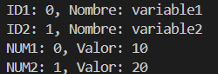
\includegraphics[width=0.5\linewidth]{image.png}
\end{figure}

Los resultados muestran que los primeros dos identificadores se almacenan correctamente en las posiciones 0 y 1 de la tabla \texttt{idTable}, con los nombres correspondientes. De igual forma, los números ingresados se ubican en las posiciones iniciales de la tabla \texttt{numTable}, confirmando que la inserción en estructuras vacías funciona como se espera y que cada elemento se indexa de manera secuencial.

\subsubsection{Escenario 2:Inserciones Adicionales }

El segundo escenario valida que se puedan añadir más registros sin afectar los existentes. El código ejecutado fue:

\begin{verbatim}
int id3 = installID("loopVar");
int num3 = installNum(30);
printf("ID3: %d, Nombre: %s\n", id3, idTable[id3].name);
printf("NUM3: %d, Valor: %d\n", num3, numTable[num3].value);
\end{verbatim}

\begin{figure}[H]
    \centering
    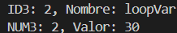
\includegraphics[width=0.5\linewidth]{image2.png}
\end{figure}

Aquí se observa que un identificador nuevo ID3 se almacena en la segunda posicion de la tabla de identificadores y un numero nuevo NUM3 es instalado en la posicion 2. Esto evidencia que el proceso de inserción respeta el orden y no sobrescribe registros previos, manteniendo la coherencia de las estructuras.
 
\subsubsection{Escenario 3: Prueba de Capacidad Máxima}

El último caso pone a prueba la limitación de espacio definida por \texttt{TABLE\_SIZE}. El fragmento ejecutado realiza múltiples inserciones hasta agotar el espacio:

\begin{verbatim}
for (int i = 0; i < TABLE_SIZE; i++) {
  installID("tempID");
  installNum(100 + i);
}
\end{verbatim}

\begin{figure}[H]
    \centering
    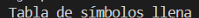
\includegraphics[width=0.5\linewidth]{image3.png}
\end{figure}

Se verifica que, una vez alcanzado el tamaño máximo, el sistema detiene las inserciones adicionales y muestra un mensaje de advertencia.

\subsubsection{Conclusiones}

Del análisis de las pruebas se destacan las siguientes observaciones:

\begin{itemize}
  \item Las funciones \texttt{installID} e \texttt{installNum} se comportan de forma correcta, gestionando la inserción secuencial de registros sin sobrescribir información.
  \item El tamaño fijo de las tablas de símbolos (\texttt{TABLE\_SIZE}) limita la cantidad de entradas, lo cual puede ser un inconveniente si se requiere manejar grandes volúmenes de datos.
  \item La implementación no contempla mecanismos para optimizar espacio, como redimensionamiento dinámico o reutilización de entradas eliminadas, lo que representa un punto de mejora para futuros ajustes.
\end{itemize}

En general, los resultados evidencian que el analizador léxico y la gestión de tablas funcionan como se diseñaron, validando la correcta categorización y almacenamiento de tokens durante el análisis.

\section{Referencias}
\renewcommand{\refname}{}
\begin{thebibliography}{9}
\bibitem{1}
Aho, A. V., Lam, M. S., Sethi, R., \& Ullman, J. D. (2007). \textit{Compilers: Principles, Techniques, and Tools} (2nd ed.). Pearson Education.
\bibitem{2}
Appel, A. W., \& Palsberg, J. (2004). \textit{Modern Compiler Implementation in Java} (2nd ed.). Cambridge University Press.
\bibitem{3}
Westes, B. (n.d.). \textit{flex: The fast lexical analyzer}. GitHub. Retrieved December 13, 2024, from \url{https://github.com/westes/flex}

\end{thebibliography}

\end{document}